\documentclass[a4paper]{article}

%% Language and font encodings
\usepackage[english]{babel}
\usepackage[utf8x]{inputenc}
\usepackage[T1]{fontenc}

%% Sets page size and margins
\usepackage[a4paper,top=3cm,bottom=2cm,left=3cm,right=3cm,marginparwidth=1.75cm]{geometry}

%% Useful packages
\usepackage{amsmath}
\usepackage{graphicx}
\graphicspath{ {images/} }

\usepackage[colorlinks=true, allcolors=blue]{hyperref}

\title{Assignment 2 - Software Requirements and Planning}
\author{ by Group 3 - Plant-Id \\* \\* Team Members: \\* Ethan Ahuja - ahujae \\* Ethan Patterson - patteret \\* James Barry - barryj \\* Evan Brass - brassev \\* Zachary Comito - comitoz \\* \\* Customers: \\* Ethan Ahuja - ahujae \\* Ethan Patterson - patteret }

\begin{document}
\maketitle
\pagebreak
\tableofcontents
\pagebreak

\section{Project Description}
Plant-Id is a mobile application that implements a decision tree to identify plant species. This is accomplished by asking the user a series of question.  With each question asked the decision tree can narrow down a large list of species to a single organism.

\subsection{Proposed System}
Plant-Id is a mobile application that can help the user identify a plant. The application will use a decision tree to ask the user questions about the plant they are observing, gradually narrowing down options until the application is able to identify the plant. It will also employ entropy in order to ask questions in the most efficient order possible. The application could also use a neural network to identify plants based on pictures taken by the user. However, creating a neural network is time consuming and likely too ambitious given the project constraints. We would also like to implement a user feedback system that will allow users to send a picture of the plant they are trying to identify if the system fails to identify it properly. Administrators could then use this information to correct errors in the database and improve its accuracy. 

Currently, a binary decision tree for identifying plants does not exist. Image recognition systems have already been implemented, however. This inherent uniqueness is how ours differs from previous approaches. User feedback and geo-tagging will also create a community that helps to upkeep the application alongside the developers. 

\subsection{Target Audience}
Those who would benefit from this application range from the casual to the professional. The curious hiker who is out in the middle of their hike comes across an intriguing plant and would like to know the name of this wonderful organism. They could learn about the plant and its origin, and also know if it is safe to pick or eat. A professional botanist might be in an area full of plant species that they are unfamiliar with and could use assistance in identifying the unknown organisms.  Additionally, we would like to include geo-tagging capabilities, meaning users can chose to send the details of their finding back to the database, mainly the location that they found it. This makes the application more useful, as botanists could use this geo-tagging information to track invasive or endangered species.

\subsection{Tools and Languages}
As stated earlier, this application will use a decision tree to identify plant species. A decision tree is a machine learning algorithm that asks binary questions to reach a conclusion. It closely follows fundamental computer science notation of divide and conquer. Every question is binary, allowing for the tree to sort through $2^N$ options, where N is the number of questions. For example, 20 questions can sift through $2^{20}$ which is 1,048,576 options. Mapping these options creates a tree-like structure with the question being a parent node and the leafs being the yes or no responses. We may implement a non-binary search tree, allowing for questions to be more open-ended, such as asking if the plant has leaves or needles, or asking how many points the leaves on the plant has. However, a non-binary decision tree is more complex to implement, so it may be outside the constraints of this project.

We will likely be creating three systems for the application. One is the server, which will contain the plant information and decision tree. It will also allow for edits and additions to the database. Second is the application that the end user will interact with.  It will run on Android and facilitate downloading the required plant information, walking the user through the decision tree, and possibly submitting new images of plants to the server and allowing users to verify plant identifications or suggest updates to the server's data. The plant data could be stored easily in an SQL database.  We may chose to including a middle-man server between the application and SQL database, which would give administrators and easy interface to make changes to the database, rather than just having them directly edit the SQL database. To create a decision tree, we need spreadsheet or tabular data, hence our decision to use SQL.  For the Android app we've decided to use Kotlin.  Between Java and Kotlin, we would rather learn Kotlin and it has full support for Android.  The last system is the image identification system.  We hope to add this later in the project so it makes sense to keep it separate from the rest of the systems.  The app would then interface with the SQL server, and a separate image identification server.

\subsection{Non-Functional Requirements and Documentation}
Ideally, we would like our decision tree to identify a plant within 20 questions in order to make it convenient for the user. We would also like a sleek and clear interface that clarifies questions to the user. For example, a question the application could ask is "Does the plant have leaves or needles?" In this circumstance, two buttons could be displayed to the user, one containing a simple vector image of needles and the other containing the same for leaves. Whether or not a question like this would be included depends on if we implement a binary decision tree or a more open-ended one. Application size is also important, so we need to optimize the amount of information stored locally on the device. Since users will often be out in the wild where there is no wi-fi or cellular signal, we will have to evaluate the practicality of storing plant information locally on the user's device.

Documentation for the application will be fairly simple, as it essentially walks the user through everything. After initializing the application, they will have a clear option to start the decision tree process, and each question will be self-explanatory. The application will be distributed on the Google Play store, so a description of the application will need to be written for it.

\pagebreak

\section{Use Cases}
\subsection{Decision tree}
\begin{itemize}
\item Goal: Identify a plant.
\item Actors: User and plant.
\item Pre-condition: Plant must be in data set.
\item Post-condition: Identifies plant to the user.
\begin{center}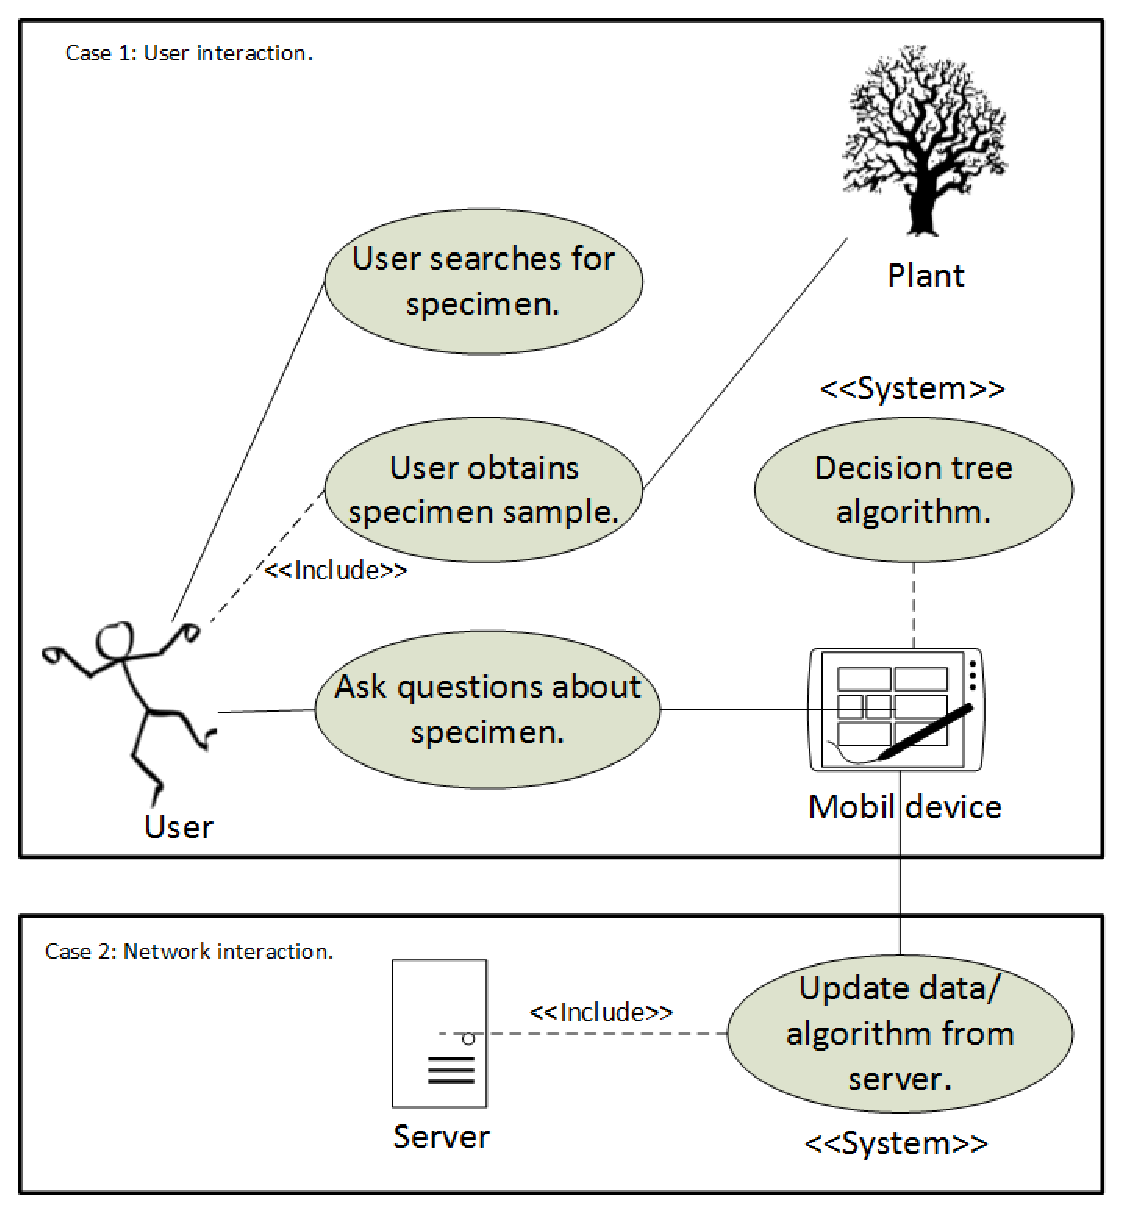
\includegraphics[scale=.8]{DecisionTree.eps}\end{center}
\end{itemize}
\pagebreak
\subsection{Geotagging}
\begin{itemize}
\item Goal: User sends plant location data to server.
\item Actor: User and plant
\item Pre-condition: Plant must be in data set.
\item Post-condition: Sends plant location to server.
\begin{center}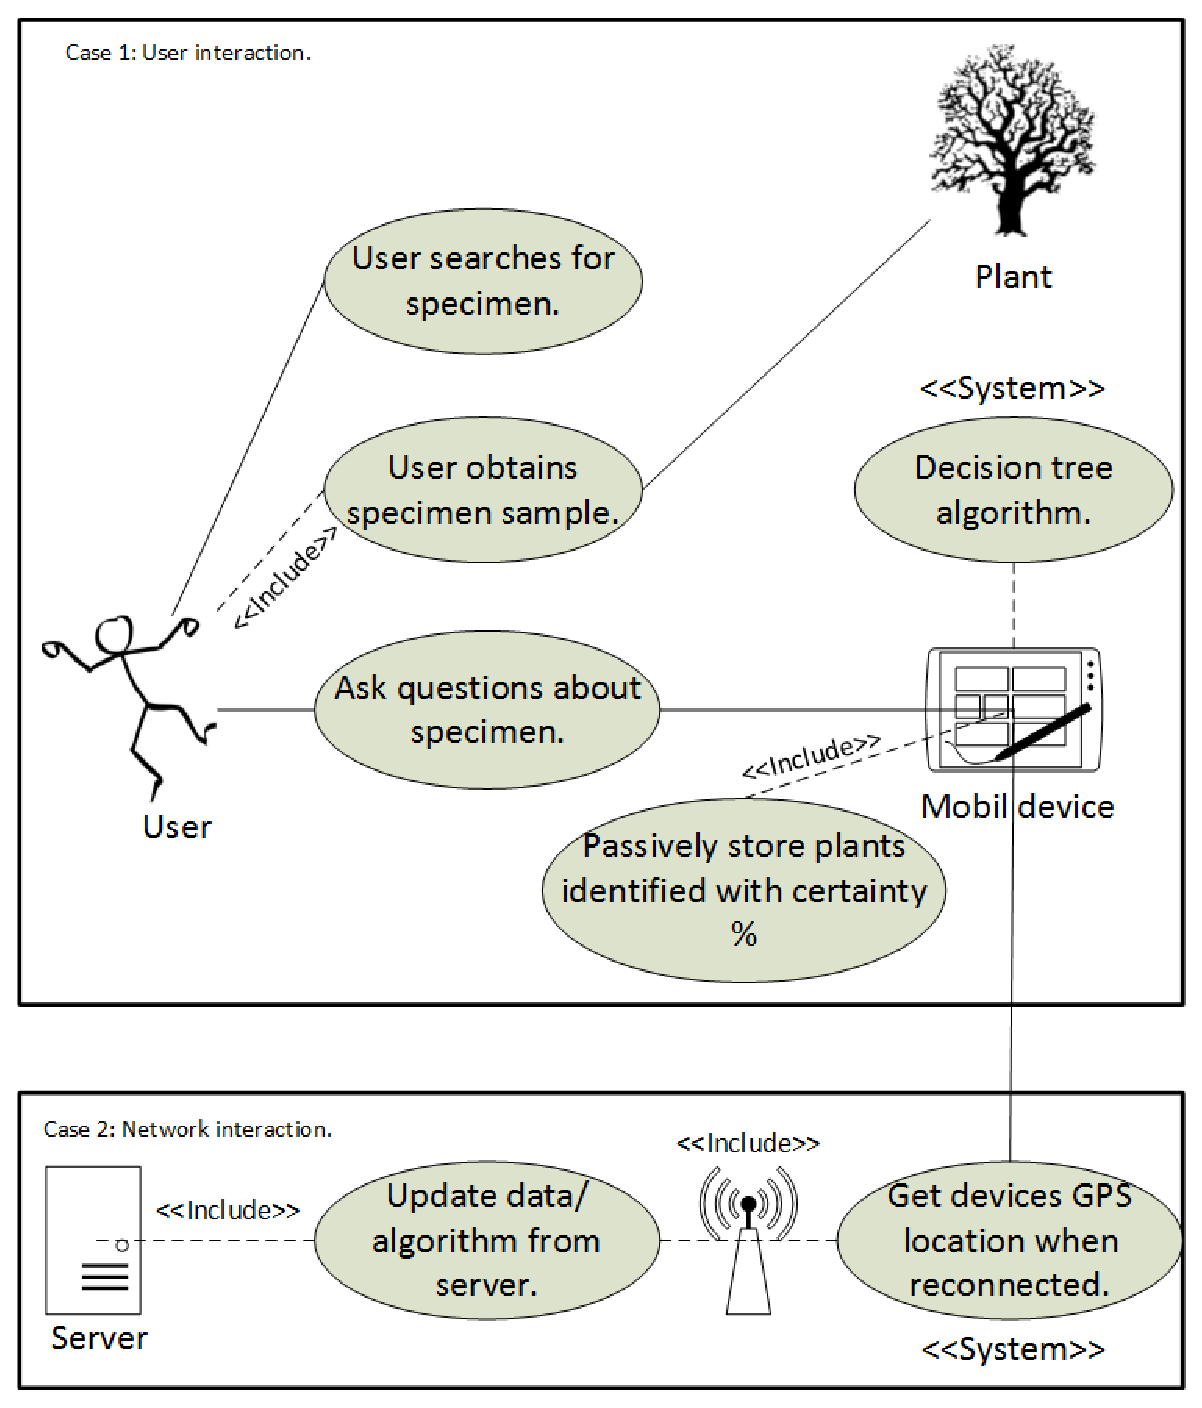
\includegraphics[scale=.8]{Geotagging.eps}\end{center}
\end{itemize}
\pagebreak
\subsection{Image Recognition}
\begin{itemize}
\item Goal: Identify a plant with a picture.
\item Actor: User and plant
\item Pre-condition: Neural net must be trained for the plant.
\item Post-condition: Identifies plant to the user.
\begin{center}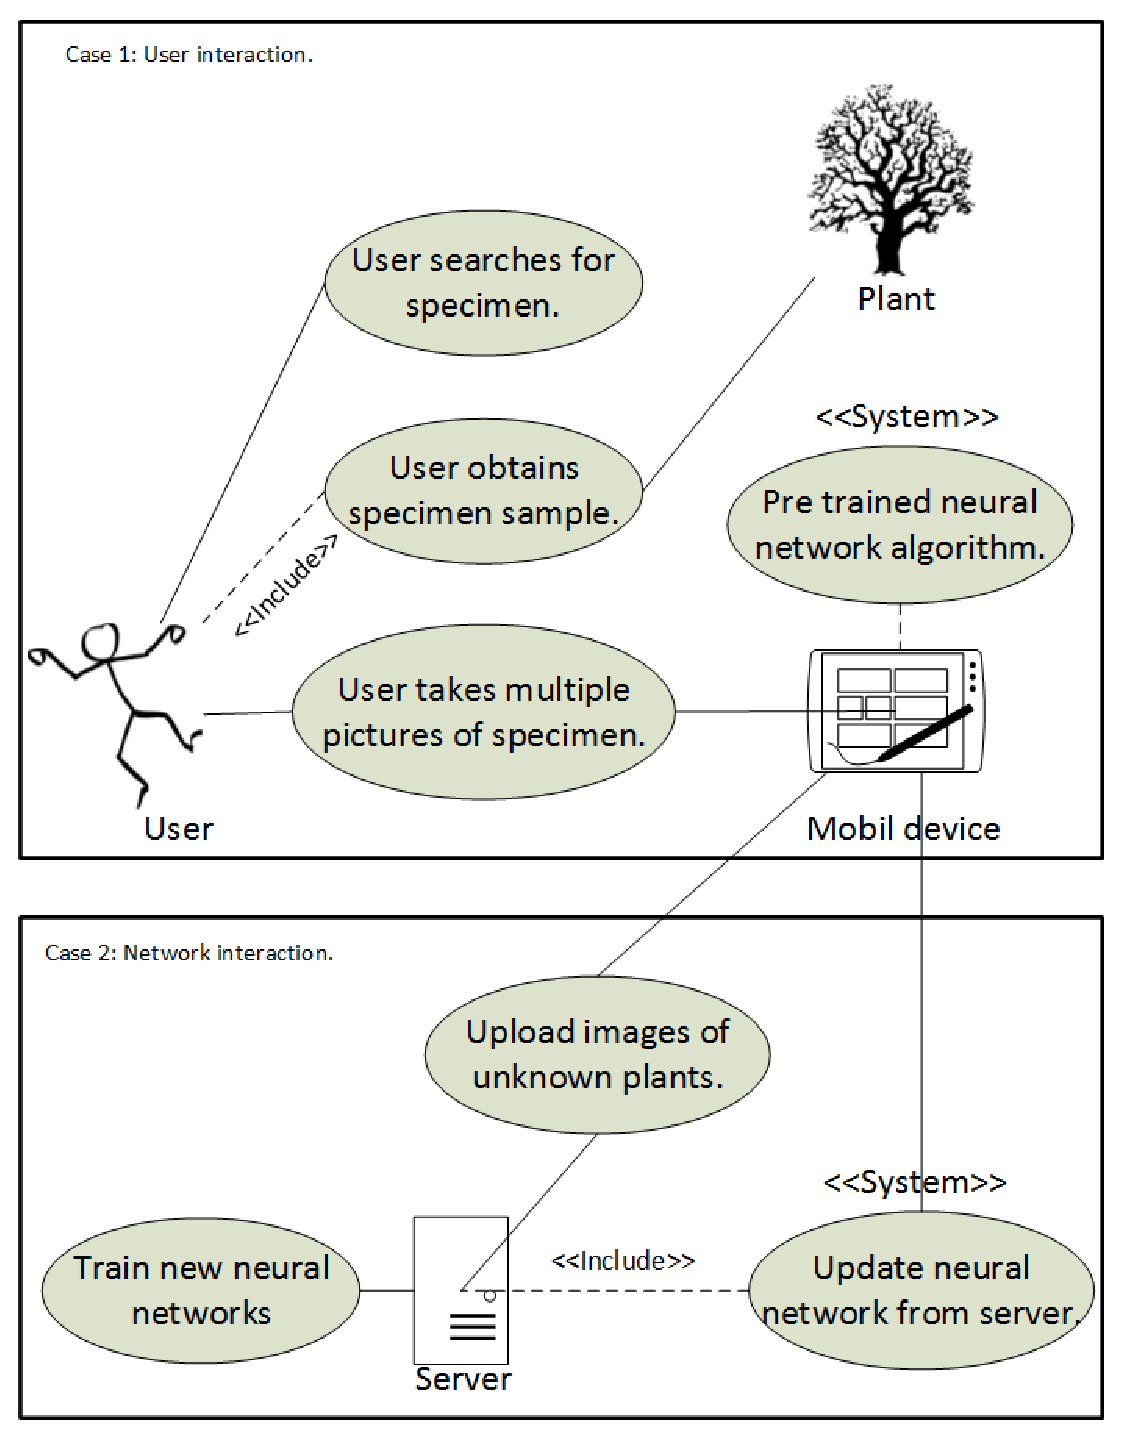
\includegraphics[scale=.8]{neuralNet.eps}\end{center}
\end{itemize}
\pagebreak
\section{Planning}
\subsection{Milestones}
\begin{enumerate}
\item Learn Kotlin, decision tree methdology
\item Create a test decision tree
\item SQL Database setup (SQL Schema defined)
\item 100 Test plants uploaded
\item Hard-coded Decision tree loaded into database
\item App traverses decision tree
\item All desired local plants setup in the database
\item Decision Tree Trained - Entropy implemented
\item Icons created for selected questions
\item Further goals\begin{enumerate}
\item App feature: Report unrecognized plant
\item App feature: Report location of plant
\item Botanist feature: Identify unidentified plant
\item App feature: Map with locations
\item App feature: Plant details page (Edible, invasive, description?)
\item Neural network training
\item Implement image identification through neural network
\end{enumerate}
\end{enumerate}
\subsection{Schedule}
We are uncertain of what the class schedule is and what our final due date will be, so our project may change slightly once we become aware of these dates. Our first goal is to have all of our project planning and requirements laid out by the end of week 3. By the end of week 4, we would like to have learned necessary info, like learning Kotlin and decision tree implementation. We would also like to have laid out our database. For week 5, we would like to design our system using UML. The following weeks (6 through 10) will be for implementing our design and going through the testing process, and then revising our system and implementation based on testing. A rough schedule for our milestones can be found below.

\begin{center}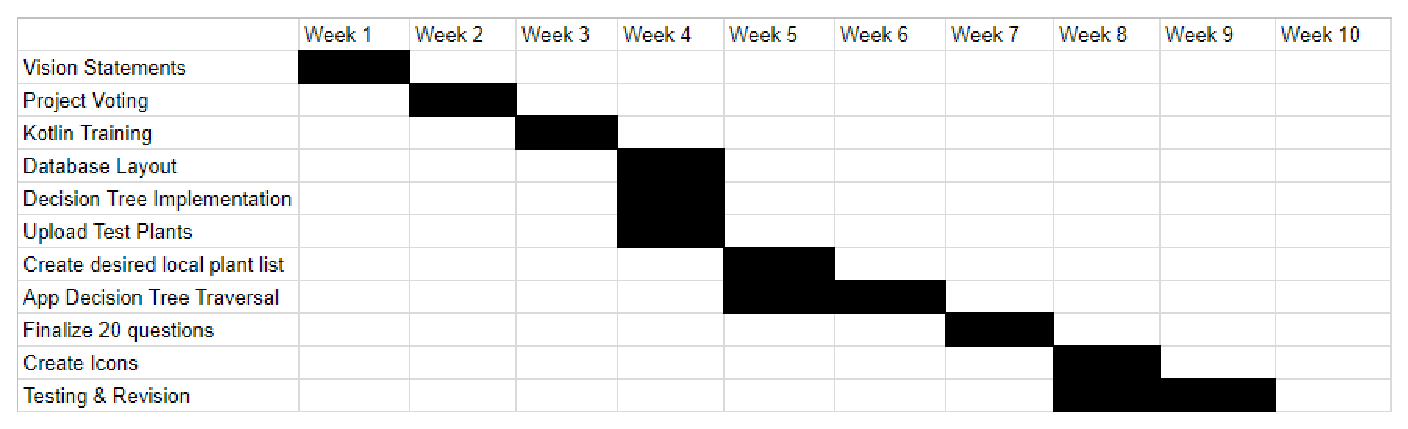
\includegraphics[width=6in]{schedule.eps}\end{center}

\subsection{Project tracking}
We will use GitHub to manage our project. Each group member will have their own branch and we will merge changes to our master branch as we move along. We will have weekly meetings in order to evaluate our progress and change our schedule if needed. Ideally, we will do most of our work during these weekly meetings, as most of the time we have to dedicate to this project is on the weekends. Any work done remotely will be evaluated during our weekly meetings. 

\subsection{Risk Management and Analysis}
(Risk) : (Likelihood) : (Plan for mitigation)
\begin{enumerate}
\item Making it look good (Icons, Artwork, Animations) : Unlikely : At most we'll have 20 pairs of graphics and we can likely find outside help.
\item Lack of knowledge about Android Development : Very Likely : We'll be studying Kotlin, and Android development this first week of the project.
\item Building a large enough dataset : Semi-Likely : We have looked into how we might be able to seed our dataset.  We may need to crawl some of the online databases from OSU's Botany department.
\item Users submitting bad data : Almost a certainty : We want to establish the functionality to support a community of experts who would moderate unidentified plants.
\item No fifth member : Semi-Likely : We have been unable to get in touch with our fifth member Zachary Comito, meaning we may have to find a fifth member or move forward with only four. 
\item Inaccuracy of botany information : Likely : None of the team members have much botany knowledge, so we must be certain to gather accurate information when creating our decision tree. Outside help, possibly from OSU's botany department, could assist in this. 
\end{enumerate}

\section{Meeting Report}
\textbf{01/27/2018 (3:00pm - 7:00pm):} Valley Library - Basement
\begin{itemize}
\item We created a rough plan of everything we need to do to complete our project. We also discussed requirements and specifications, as well as created some use cases to further clarify the features of the application. 
\item By next week, we want to get a test decision tree implemented as well as our SQL database laid out. We would also like to have learned Kotlin so that we can properly implement our program. 
\item Ethan Patterson created all of the use cases and the diagrams for them. The other three members at the meeting (James Barry, Evan Brass, Ethan Ahuja) discussed and completed the rest of the above document. Zachary Comito did not attend the meeting, as we have been unable to contact him.
\item Our customers were perfectly willing to meet with us and contributed to the assignment appropriately.
\end{itemize}

\newpage %Move references to the next page..
\begin{thebibliography}{9}
\bibitem{latexcompanion} 
\url{http://www.saedsayad.com/decision_tree.htm}
Dr. Saed Sayad, Reading, www, 2010-2018.
\bibitem{einstein} 
Victor Lavrenko.
\url{https://www.youtube.com/watch?v=eKD5gxPPeY0&list=PLBv09BD7ez_4temBw7vLA19p3tdQH6FYO}
\textit{School of Informatics} 
[\textit{Decision Trees}]. 
Victor Lavrenko and Nigel Goddard, January 19, 2014.
\end{thebibliography}
\end{document}